\documentclass[a4paper,12pt,titlepage]{article}
\usepackage[utf8]{inputenc}
\usepackage{graphicx} % Required for inserting images
\usepackage[spanish,es-tabla]{babel}
\usepackage[none]{hyphenat}
\usepackage[justification=centering]{caption}
\usepackage{subcaption}
\usepackage{amssymb, amsmath}
\usepackage{gensymb}
\usepackage{fancyhdr}
\usepackage{wrapfig}
\usepackage{physics}

\usepackage[a4paper]{geometry}
\geometry{top=3cm, bottom=3.0cm,left=2cm, right=2cm}


\lhead{Densidad en sistemas binarios}
\rhead{Gonzalo Bastos González}

\pagestyle{fancy}

\title{Densidad en sistemas binarios}
\author{Gonzalo Bastos González}
\date{Técnicas expermimentales II-Laboratorio de termodinámica}

\begin{document}

\maketitle
\tableofcontents

\newpage

\section{Objetivos e introducción teórica}

El objetivo de esta práctica es el estudio de un sistema binario agua-etanol, para obtener así una relación entre la densidad y la concentración de las especies químicas. Para ello tomaremos diferentes medidas de la densidad a temperaturas y concentraciones diferentes, $\rho(x,T)$. Tomadas estas medidas fijaremos una temperatura de trabajo, $T_0$, para la que vamos a determinar una expresión para $\rho(x)$. Una vez conocida esta relación vamos a calcular diferentes volúmenes de la mezcla; el volumen de exceso, el volumen aparente y el volumen molar parcial.

\subsection{Preparación de las mezclas}

La base teórica de esta práctica es el concepto de densidad además del concepto de fracción molar, por estar trabajando en un sistema binario, con dos componentes:

\begin{equation}
    \rho = \frac{m}{V} \quad x_i=\frac{n_i}{n_T}
\end{equation}

En nuestra práctica tomamos como valor de referencia la fracción molar de agua, que es la que emplearemos de ahora en adelante y tiene la siguiente expresión:

\begin{equation}
    \chi_{H_20} = \frac{n_{H_20}}{n_{H_20}+n_{OH}}
\end{equation}

Donde el subíndice $OH$ hace referencia al etanol. Una forma más cómoda de expresar la fracción molar, en función de las masas y molaridades, es la siguiente:

\begin{equation}
    \chi_{H_2O} = \frac{1}{1+\frac{m_{OH}M_{H_2O}}{m_{H_2O}M{OH}}}
    \label{x_agua}
\end{equation}

Donde $M_i$ hace referencia a la masa molar de cada sustancia. Como en el laboratorio podemos medir masas y no moles empleamos la siguiente relación para determinar la masa de agua que llevará una determinada muestra con una $x_{H_2O}$ arbitraria:

\begin{equation}
    m_{H_20} = \frac{m_T}{1+\frac{M_{OH}}{M_{H_2O}}\left(\frac{1}{\chi_{H_2O}}-1\right)}
    \label{m_agua}
\end{equation}

Esta expresión nos será útil a la hora de preparar las diferentes muestras. Un aspecto importante a la hora de la preparación de las muestras es que estamos trabajando con etanol-96, es decir, la sustancia que empleamos está formada por un 96\% de etanol y un 4\% de agua en volumen. Por tanto, tendremos que realizar una corrección, que detallaremos más adelante, en el apartado de la metodología.

\subsection{Volúmenes molares}

Otra parte de la práctica es el estudio de diferentes volúmenes molares, el volumen de exceso, el volumen aparente y el volumen parcial para cada concentración.

\subsubsection{Volumen molar de exceso}

El concepto de volumen de exceso está asociado a la mezcla de diferentes fases en un mismo sistema. En nuestro caso tendremos dos fases, el etanol y el agua, que antes de mezclarse presentarán un volumen:

\begin{equation}
    V^0 = n_{H_2O}V_{H_2O}^0 + n_{OH}V_{OH}^0
    \label{V_exc}
\end{equation}

Una vez hecha la mezcla los volúmenes van a variar, por lo que para ello definimos los volúmenes molares parciales de los componentes, $\Bar{v}_i$ como las magnitudes que verifican:

\begin{equation}
    V = n_{H_2O}\Bar{v}_{H_2O} + n_{OH}\bar{v}_{OH}
\end{equation}

Donde $V$ es el nuevo volumen que adopta la mezcla. El volumen de mezcla, $V^M$, se define como la variación de volumen que se da durante el proceso de mezcla:

\begin{equation}
    V^M = V-V^0= n_{H_2O}(\Bar{v}_{H_2O}-v_{H_2O}^0) - n_{OH}(\Bar{v}_{OH}-v_{OH}^0)
\end{equation}

Se define ahora el volumen de exceso como la diferencia entre el volumen de mezcla real y el volumen de mezcla en caso de que el sistema se comportase idealmente:

\begin{equation}
    V^{E} = V^M - V^{M,id}
\end{equation}

Sabemos que el volumen de mezcla de los sistema que se comportan idealmente es nulo, el volumen del producto final es la suma de los volúmenes iniciales. Por tanto, podemos identificar el volumen de exceso con el volumen de mezcla en todos los casos. El volumen molar de exceso se puede escribir como:

\begin{equation}
    v^{E} = \frac{V^M}{n} = \frac{V}{n} - (x_{H_2O}v_{H_2O}^0 + x_{OH}v_{OH}^0)
\end{equation}

Donde $x_i=n_i/n$ es la fracción molar de cada una de las componentes. No obstante, no podemos medir los moles, por lo que es muy cómodo expresar el volumen molar de exceso en función de las densidades a partir de las siguientes relaciones:

\begin{equation}
    \begin{gathered}
        V=\frac{m}{\rho} = \frac{M_{H_20} + M_{OH}}{\rho} = \frac{n_{H_2O}M{H_2O} + n_{OH}M_{OH}}{\rho} \\
        V_i^0 = \frac{M_i}{\rho_0}
    \end{gathered}
\end{equation}

Donde $\rho^0_i$ es la densidad del componente $i$ puro. Entonces, podemos expresar el volumen molar de exceso como:

\begin{equation}
    v^{E} = \frac{x_{H_2O}M{H_2O} + x_{OH}M_{OH}}{\rho} - \left( \frac{x_{H_2O}M_{H_2O}}{\rho_{H_2O}^0} + \frac{x_{OH}M_{OH}}{\rho_{OH}^0} \right)
\end{equation}

La incertidumbre del volumen molar de exceso se puede obtener por propagación a partir de la siguiente expresión:

\begin{equation}
    s(v^{E}) = \sqrt{A^2 s^2(\chi_{H_2O}) + B^2 s^2(\chi_{OH}) + C^2 s^2(\rho) + D^2 s^2(\rho_{H_2O}) + E^2 s^2(\rho_{OH})}
    \label{s_vE}
\end{equation}

Escrita de forma abreviada, los coeficientes se corresponden con las parciales:

\begin{equation}
    \begin{gathered}
        A = \left( \pdv{v^{E}}{\chi_{H_2O}} \right) =  \frac{M_{H_2O}}{\rho} - \frac{M_{H_2O}}{\rho_{H_2O}} \quad B = \left( \pdv{v^{E}}{\chi_{OH}} \right) = \frac{M_{OH}}{\rho} - \frac{M_{OH}}{\rho_{OH}} \\
        C = \left(\pdv{v^E}{\rho}\right) = -\frac{x_{H_2O}M{H_2O} + x_{OH}M_{OH}}{\rho^2} \\
        D = \left(\pdv{v^E}{\rho_{H_2O}}\right) = -\chi_{H_2O}\frac{M_{H_2O}}{\rho^2_{H_2O}} \quad E = \left(\pdv{v^E}{\rho_{Oh}}\right) = -\chi_{OH}\frac{M_{OH}}{\rho^2_{OH}}
    \end{gathered}
\end{equation}

\subsubsection{Volumen molar aparente}

El volumen molar aparente es otra forma de estudiar el cambio del volumen que se da tras un proceso de mezcla. Podemos adjudicar todo ese cambio del volumen al soluto, definiendo el volumen molar aparente, $v_{\phi)}$,  como aquel que verifica:

\begin{equation}
    V = n_1v_1^0 + n_2v_{\phi}
\end{equation}

Considerando la magnitud 1 como disolvente y la 2 como soluto. Despejando, podemos expresar este volumen aparente como:

\begin{equation}
    v_{\phi} = \frac{V}{n_2} - \frac{n_1v_1^0}{n_2} = \frac{m_1}{\rho n_2} + \frac{m_2}{\rho n_2} - \frac{m_1}{\rho_1^0 n_2} = \frac{M_2}{\rho} + \frac{1}{m} \frac{\rho_1^0 - \rho}{\rho \rho_1^0}
\end{equation}

Siendo $1/m$ la inversa de la molalidad. La incertidumbre del volumen molar aparente viene dada por la siguiente expresión:

\begin{equation}
    s(v_{\phi}) = \sqrt{A^2 s^2(m) + B^2s^2(\rho_1^0) + C^2s^2(\rho)}
\end{equation}

Donde los coeficientes son otra vez las parciales:

\begin{equation}
    \begin{gathered}
        A = \left( \pdv{v_{\phi}}{m} \right) = \frac{-1}{m^2} \frac{\rho_1^0 - \rho}{\rho \rho_1^0} \quad\quad
        B = \left( \pdv{v_{\phi}}{\rho_1^0} \right) = \frac{-1}{m} \frac{1}{(\rho_1^0)^2} \quad\quad
        C = \left( \pdv{v_{\phi}}{\rho} \right) = \frac{-M_2}{\rho^2} - \frac{1}{m} \frac{1}{\rho^2}
    \end{gathered}
\end{equation}

\subsubsection{Volumen molar parcial}

Los volúmenes molares parciales se definen como las derivadas parciales de la Ec.\ref{V_exc}. En concreto para el soluto es muy cómodo emplear la relación del volumen aparente obtenida anteriormente:

\begin{equation}
    \Bar{v}_2 = \left(\pdv{V}{n_2} \right)_{T,P} = v_{\phi} + n_2 \left( \pdv{v_{\phi}{n_2}} \right)_{T,P} = v_{\phi} + m\left( \pdv{v_{\phi}{m}} \right)_{T,P}
\end{equation}

Donde $m$ es la molalidad otra vez. El último paso viene de la definición de molalidad y de aplicar la regla de la cadena, $m=n_2/m_1$, $\partial/\partial m = (\partial/\partial n_2/m)$.
Durante el tratamiento de datos estudiaremos los casos en la que el agua y el etanol se suponen los solutos. Si desarrollamos esta expresión para nuestros casos concretos llegamos a una expresión mucho más simple para los volúmenes molares parciales y su incertidumbre:

\begin{equation}
        \Bar{v}_2 = \frac{M_2}{\rho} \quad \quad
        s(\Bar{v}_2) = \frac{M_2}{\rho^2} s(\rho)
\end{equation}


\section{Materiales y procedimiento experimental}

\subsection{Material empleado}

El material empleado durante la práctica fue el siguiente:

\begin{itemize}
    \item 11 frascos con su respectiva preparación del sistema binario
    \item Baño de agua caliente
    \item Balanza para preparar las muestras
    \item Densímetro digital
    \item Jeringuillas y pipetas
\end{itemize}

El densímetro es el principal instrumento de medida que emplearemos, nos proporcionará el valor de la densidad y la temperatura del líquido que introduzcamos en su interior, obteniendo así nuestros pares de valores $(\rho,T)$ que emplearemos a lo largo de la práctica. Su funcionamiento está basado en un diapasón que oscila en su interior por el que circula el líquido. Si modelizamos el movimiento del diapasón como un oscilador armónico simple podemos afirmar que tiene un período:

\begin{equation}
    T = 2\pi \sqrt{\frac{m}{k}}
    \label{Densimetro}
\end{equation}

Donde la masa del oscilador vendrá dada por:

\begin{equation}
    m = m_0 + \rho V
\end{equation}

Donde $m_0$ es la masa del tubo vacío y $\rho$ y $V$ son las magnitudes referidas al líquido a estudiar. Como $m_0$ y $V$ son magnitudes constantes podemos afirmar que $T=T(\rho)$. Operando con la expresión (\ref{Densimetro}) podemos llegar a la siguiente expresión para la densidad:

\begin{equation}
    \rho = \frac{T^2-A}{B}
\end{equation}

Donde $A$ y $B$ son dos constantes que se pueden calcular con dos sustancias conocidas, normalmente el agua y el aire. Nuestro densímetro está equipado para medir ya directamente la densidad y la temperatura de la muestra que circula por el interior.

\subsection{Cálculos previos}

Antes de empezar a preparar las muestras tenemos que realizar ciertos cálculos para saber las cantidades que debemos mezclar de cada una de las sustancias. En primer lugar realizaremos los cálculos tomando que estamos trabajando con etanol puro, pese a que estamos trabajando con etanol-96. Una vez tengamos los cálculos realizaremos la corrección correspondiente, que detallaremos más adelante.

Para un estudio en profundidad prepararemos 11 mezclas con fracciones molares de agua variando de 0 a 1, en intervalos de 0,1. Empleando la expresión (\ref{m_agua}) obtenemos las masas de agua teóricas que le corresponden a nuestras diferentes fracciones molares. Para la preparación de las muestras tomamos como referencia un valor para la masa total de las muestras de 20 g pero que variará de una muestra a otra, como se verá en la tabla de los datos. Una vez conocidos los valores teóricos de las masas podemos realizar las correcciones correspondientes.

\begin{table}[h!]
\centering
\begin{tabular}{|c|c|c|c|}
\hline
$\chi_{H_2O}$ & $m_{H_2O} \;(g)$  & $m_{OH}\;(g)$ & $m_T\;(g)$ \\ \hline
0     & 0      & 20,000 & 20,000  \\ \hline
0,1   & 0,833  & 19,167 & 20,000  \\ \hline
0,2   & 1,782  & 18,218 & 20,000  \\ \hline
0,3   & 2,872  & 17,128 & 20,000  \\ \hline
0,4   & 4,138  & 15,862 & 20,000  \\ \hline
0,5   & 5,625  & 14,375 & 20,000  \\ \hline
0,6   & 7,397  & 12,603 & 20,000  \\ \hline
0,7   & 9,545  & 10,455 & 20,000  \\ \hline
0,8   & 12,203 & 7,797  & 20,000  \\ \hline
0,9   & 15,577 & 4,423  & 20,000  \\ \hline
1     & 20,000 & 0      & 20,000  \\ \hline
\end{tabular}
\caption{Masas teóricas de etanol y agua}
\label{tab:my-table}
\end{table}

\subsection{Preparación de las muestras y cálculo de las masas reales}

Como ya hemos mencionado anteriormente, estamos trabajando con etanol-96 en todo momento. Esto significa que el 96\% del volumen es etanol, mientras que el otro 4\% es agua. Para trabajar con las cantidades de cada sustancia tenemos que tener esto en cuenta durante la preparación de las muestras.

El proceso llevado a cabo fue el siguiente:

\begin{enumerate}
    \item Colocamos el frasco en la balanza, taramos y añadimos la masa de agua teórica.
    \item Añadimos alcohol con la jeringuilla hasta acercarnos a los 20 g.
    \item Añadimos alcohol de forma más precisa con la pipeta hasta llegar a 20 g más o menos.
    \item Cerramos la muestra y recalculamos la fracción molar real.
\end{enumerate}

La incertidumbre de las masas que estamos midiendo continuamente viene siempre dada por la precisión experimental de la balanza, $s(m)=0,001\;g$. Para la corrección partimos de que la masa de etanol-96 es:

\begin{equation}
    \begin{gathered}
        m_{96} = m_T-m_{H_2O} \\
        s(m_{96}) = \sqrt{\left(\pdv{m_{OH}}{m_T}\right)^2s(m)^2+\left(\pdv{m_{OH}}{m_{H_2O}}\right)^2s(m)^2} = \sqrt{2}s(m) = 0,0014 \;g
    \end{gathered}
\end{equation}

El volumen del etanol empleado es:

\begin{equation}
    V_{96} = V_{H_2O} + V_{OH} = \frac{m_{H_2O}}{\rho_{H_2O}} + \frac{m_{OH}}{\rho_{OH}}
\end{equation}

Como conocemos la composición en volumen del etanol podemos calcular la masa de etanol puro y agua que hay en el etanol-96. Para ello emplearemos las siguientes densidades teóricas de las sustancias:

\begin{equation}
    \rho_{H_2O} = \;1g/cm^3 \quad \rho_{OH} = 0,789 \;g/cm^3 \quad \rho_{96} = 0,805 \;g/cm^3
\end{equation}

La masa de cada uno de los componentes del etanol-96 es:

\begin{equation}
    \begin{gathered}
        m_{OH,96} \equiv m_{OH} = 0,96m_{96}\frac{\rho_{OH}}{\rho_{96}} \\
        m_{H_2O,96} = 0,04m_{96}\frac{\rho_{H_2O}}{\rho_{96}}
    \end{gathered}
\end{equation}

Por tanto, la masa real de agua será:

\begin{equation}
    m_{M_2O,T} = m_{H_2O} + m_{H_2O,96}
\end{equation}

Las incertidumbres con las masas con las que trabajaremos, las masas totales de cada sustancia, son:

\begin{equation}
    \begin{gathered}
        s(m_{H_2O,T}) = \sqrt{\left(\pdv{m_{H_2O,T}}{m_{H_2O}}\right)^2 s(m)^2 + \left(\pdv{m_{H_2O,T}}{m_{H_2O,96}}\right)^2 s(m_{H_2O,96})^2}  \\
        s(m_{H_2O,T})= s(m)\sqrt{1+2\left(0,04\frac{\rho_{H_2O}}{\rho_{96}}\right)^2} = 0,0010 \;g \\
        s(m_{OH}) = \left( \pdv{m_{OH}}{m_{96}}\right) s(m_{96}) = 0,96\frac{\rho_{OH}}{\rho_{96}}s(m_{96}) = 0,0013 \;g
    \end{gathered}
\end{equation}

Para recalcular la concentración molar empleamos la expresión \ref{x_agua}, que expresaremos en función de las masas efectivas:

\begin{equation}
    \chi_{H_2O} = \frac{1}{1+\frac{m_{OH,T}M_{H_2O}}{m_{H_2T,T}M_{OH}}}
\end{equation}

La incertidumbre de esta nueva fracción molar se puede obtener por propagación:

\begin{equation}
    \begin{gathered}
    s(\chi_{H_2O}) = \sqrt{\left(\pdv{\chi_{H_2O}}{m_{OH,T}}\right)^2s(m_{OH,T})^2 + \left(\pdv{\chi_{H_2O}}{m_{H_2O,T}}\right)^2 s(m_{H_2O,T)^2}} \\
    s(\chi_{H_2O}) = \frac{M_{OH}M_{H_2O}}{\left( m_{H_2O,T}M_{OH} + m_{OH,T}M_{H_2O}\right)^2} \sqrt{m^2_{H_2O,T}s(m_{OH,T})^2+m^2_{OH}s(m_{H_2O,T})^2}
    \end{gathered}
\end{equation}

Como podemos ver, esta incertidumbre va a ser variable, dependerá de las diferentes masas de cada sustancia con la que estemos trabajando en cada momento. Incluiremos los diferentes valores de la incertidumbre en la tabla de datos que se adjuntará a continuación.

Además de la corrección del etanol-96, nosotros tuvimos un error en el cálculo teórico de las masas que requería cada fracción molar, por lo que obtuvimos valores de $\chi_{H_2O}$ totalmente diferentes a los teóricos que pretendíamos obtener. A pesar de todo, la validez de los datos sigue vigente, lo ideal sería tener puntos distribuidos de forma equidistante pero el comportamiento general debería ser el mismo. En la siguiente tabla podemos ver las masas que empleamos nosotros con el cálculo erróneo, la fracción que pretendíamos obtener y la fracción con la que realmente trabajamos, incluidas ambas correcciones.

\begin{table}[h!]
\centering
\begin{tabular}{|c|c|c|c|c|c|}
\hline
$\chi_{H_2O}$ teórica & $m_{H_2O} \;(g)$ & $m_{OH}\;(g)$ & $m_T\;(g)$ & $\chi_{H_2O,R}$, resultante & $s(\chi_{H_2O,R})$ \\ \hline
0,0                     & 1,024            & 19,390        & 20,404     & 0,11891                     & 0,00010            \\ \hline
0,1                   & 3,100            & 16,922        & 20,022     & 0,320397                    & 0,000072           \\ \hline
0,2                   & 5,032            & 15,040        & 20,072     & 0,463022                    & 0,000054           \\ \hline
0,3                   & 6,934            & 13,117        & 20,051     & 0,576825                    & 0,000043           \\ \hline
0,4                   & 8,998            & 11,169        & 20,167     & 0,675129                    & 0,000036           \\ \hline
0,5                   & 11,237           & 9,241         & 20,478     & 0,758295                    & 0,000029          \\ \hline
0,6                   & 12,703           & 7,364         & 20,067     & 0,816548                    & 0,000028           \\ \hline
0,7                   & 14,444           & 5,560         & 20,004     & 0,870205                    & 0,000027           \\ \hline
0,8                   & 16,299           & 3,743         & 20,042     & 0,918280                    & 0,000026           \\ \hline
0,9                   & 18,102           & 1,919         & 20,021     & 0,960553                    & 0,000025           \\ \hline
1,0                     & 20,211           & 0,000             & 20,211     & 1,000000                    & 0,000022           \\ \hline
\end{tabular}
\caption{Fracciones molares reales con las que trabajamos}
\label{tab:my-table}
\end{table}


Una vez recalculadas las concentraciones y preparadas las muestras las vamos introduciendo en el baño térmico para aumentar la temperatura de nuestros sistemas hasta unos $35^{\circ}C$. Una vez las muestras estén a la temperatura adecuada podemos proceder a realizar las medidas con el densímetro. El procedimiento a seguir será el mismo con todas las muestras, introduciremos una cierta cantidad de líquido en el densímetro con una jeringuilla y tomaremos varios pares de medidas de $(\rho,T)$, cada $0,5^{\circ}C$, mientras baja la temperatura hasta unos $27^{\circ}C$. Es especialmente importante tener en cuenta a la hora de realizar las medidas que el diapasón debe contener únicamente el líquido a estudiar, la presencia de líquidos de otra fracción molar y especialmente de burbujas puede afectar mucho a las medidas de densidades.


\section{Resultados experimentales y tratamiento de datos}

\subsection{Datos experimentales de $\rho(\chi,T)$}

Una vez detallado el procedimiento experimental y los pasos previos de la preparación de las muestras es hora de exponer los resultados experimentales. En la siguiente tabla podemos ver las medidas de la densidad para las once muestras a diferentes temperaturas:

\newpage

\begin{table}[h!]
\centering
\begin{tabular}{|c|c|c|c|c|c|c|c|c|}
\hline
$\downarrow \chi_{H_2O} / T\;(^{\circ}C) \rightarrow$ & 30,5   & 30,0   & 29,5   & 29,0   & 28,5   & 28,0   & 27,5   & 27,0   \\ \hline
1,000000                                              & 0,9892 & 0,9893 & 0,9895 & 0,9896 & 0,9898 & 0,9899 & 0,9901 & 0,9902 \\ \hline
0,960553                                              & 0,9796 & 0,9798 & 0,9800 & 0,9801 & 0,9803 & 0,9804 & 0,9805 & 0,9806 \\ \hline
0,918280                                              & 0,9656 & 0,9658 & 0,9660 & 0,9663 & 0,9665 & 0,9666 & 0,9665 & 0,9667 \\ \hline
0,870205                                              & 0,9501 & 0,9504 & 0,9506 & 0,9508 & 0,9511 & 0,9515 & 0,9519 & 0,9520 \\ \hline
0,816548                                              & 0,9365 & 0,9368 & 0,9371 & 0,9373 & 0,9375 & 0,9378 & 0,9381 & 0,9385 \\ \hline
0,758295                                              & 0,9183 & 0,9186 & 0,9189 & 0,9192 & 0,9195 & 0,9198 & 0,9202 & 0,9207 \\ \hline
0,675129                                              & 0,8971 & 0,8975 & 0,8978 & 0,8982 & 0,8986 & 0,8990 & 0,8987 & 0,8992 \\ \hline
0,576825                                              & 0,8727 & 0,8731 & 0,8735 & 0,8742 & 0,8744 & 0,8748 & 0,8750 & 0,8754 \\ \hline
0,463022                                              & 0,8535 & 0,8539 & 0,8543 & 0,8546 & 0,8550 & 0,8554 & 0,8559 & 0,8563 \\ \hline
0,320397                                              & 0,8420 & 0,8426 & 0,8429 & 0,8429 & 0,8430 & 0,8430 & 0,8430 & 0,8430 \\ \hline
0,11891                                               & 0,8321 & 0,8323 & 0,8324 & 0,8326 & 0,8329 & 0,8331 & 0,8333 & 0,8334 \\ \hline
\end{tabular}
\caption{Datos experimentales de $\rho(\chi_{H_2O},T)$}
\label{tab:my-table}
\end{table}

Las densidades reflejadas en la tabla se expresan en $g\cdot cm^{-3}$. Las incertidumbres de los datos de $\rho$ y de $T$ vienen dadas por la precisión del densímetro, $s(\rho)=0,0001\; g\cdot cm^{-3}$ y $s(T)=0,1\; ^{\circ C}$. Si representamos gráficamente los datos podemos ver claramente la tendencia, la densidad es directamente proporcional a la fracción molar de agua e inversamente proporcional a la temperatura:

\begin{figure}[h!]
    \centering
    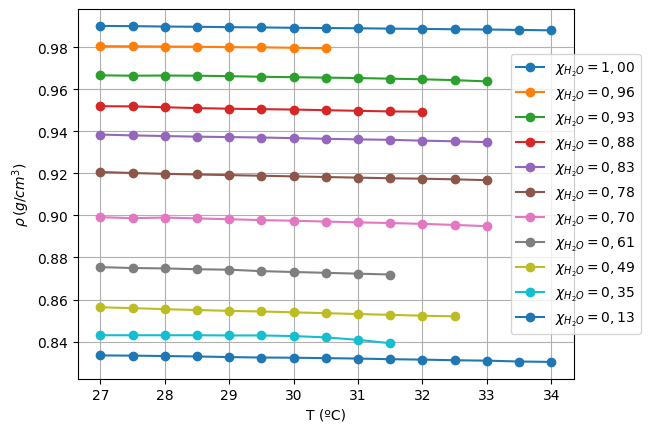
\includegraphics[width=0.75\linewidth]{Densidad/rho-T.png}
    \caption{Datos experimentales de $\rho(\chi,T)$}
    \label{fig:enter-label}
\end{figure}

Otro de los objetivos de la práctica es obtener una expresión analítica para $\rho(\chi)$. Para ello, como ya hemos mencionado antes, fijaremos una isoterma sobre la que realizar el ajuste, que denominaremos temperatura de trabajo, $T_0$.

Para escoger una temperatura de trabajo hemos probado diferentes funciones, llegando a la conclusión de que la más se ajusta es un polinomio de segundo grado del tipo $\rho(\chi) = a\chi^2 + b\chi + c$. Después de hacer una comparación entre todas las temperaturas hemos escogido la isoterma de $28 \;^{\circ}C$, que es la que más se ajusta a nuestros datos. Tomando esta temperatura de trabajo como referencia el polinomio obtenido es:

\begin{equation}
    \begin{gathered}
        \rho(\chi) = 0,1999\chi^2 - 0,041\chi + 0,8344\\
        s(a) = 0,010 \; g\cdot cm^{-3} \quad s(b) = 0,013 \; g\cdot cm^{-3} \quad s(c)= 0,0034 \; g\cdot cm^{-3}
    \end{gathered}
\end{equation}

\begin{figure}[h!]
    \centering
    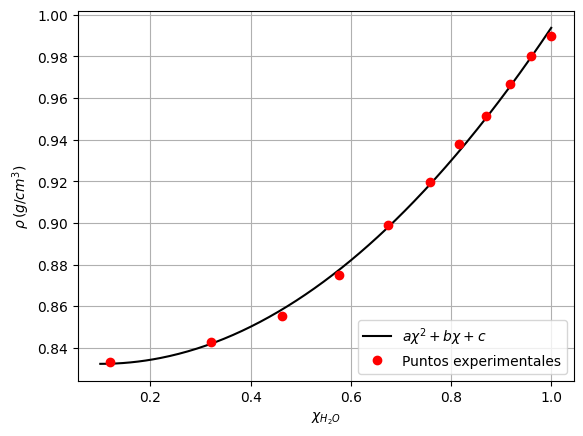
\includegraphics[width=0.65\linewidth]{Densidad/rho-x.png}
    \caption{$\rho(\chi) = 0,1999\chi^2 - 0,041\chi + 0,8344$}
    \label{fig:enter-label}
\end{figure}

Una buena forma de estudiar la validez de nuestro polinomio es analizar como se comporta en los casos límites, en nuestro caso vamos a evaluar $\rho(0)$ y $\rho(1)$:

\begin{equation}
    \begin{gathered}
        \rho(0) = c = 0,8344 \; g\cdot cm^{-3} \\
        \rho(1) = a+b+c = 0,9937 \; g \cdot cm^{-3}
    \end{gathered}
\end{equation}

Si comparamos con los valores teóricos de la densidad de ambas sustancias podemos ver que el valor de la del etanol puro se aleja bastante de lo esperado, la densidad teórica del etanol a temperatura ambiente es de $0,7893 \;g\cdot cm^{-3}$. Esto se puede explicar teniendo en cuenta la escasez de datos que hay para valores bajos de fracción molar de agua, ya que el error en los cálculos y la corrección del etanol-96 hacen que se acumulen las medidas entorno a fracciones altas. Por otro lado, el valor de la densidad del agua es mucho más acertado ya que el valor teórico a $28 \;^{\circ}C$ es de  $0,9962 \;g\cdot cm^{-3}$, apenas difiere en la tercera cifra decimal. La mayor precisión de esta medida se explica también desde la acumulación de medidas entorno a fracciones próximas a 1, que proporciona una mejor aproximación de la densidad real.


\subsection{Volúmenes molares}

\subsubsection{Volumen molar de exceso}

Como ya hemos explicado antes, el volumen molar de exceso se define como:

\begin{equation}
    v^{E} = \frac{\chi_{H_2O}M{H_2O} + \chi_{OH}M_{OH}}{\rho} - \left( \frac{\chi_{H_2O}M_{H_2O}}{\rho_{H_2O}^0} + \frac{\chi_{OH}M_{OH}}{\rho_{OH}^0} \right)
\end{equation}

Este volumen representa la desviación de la idealidad de la mezcla y depende de la densidad de la mezcla y de las diferentes fracciones molares de compuesto que está contenga. Además de eso también se tiene en cuenta el valor teórico de las sustancias puras, para el que tomaremos los valores tabulados del etanol-96 y del agua. Para estos últimos valores podríamos tomar también los valores de nuestro ajuste $\rho(\chi)$ pero creemos que debido a la notable desviación del valor de la densidad del etanol-96 respecto al valor teórico era más apropiado tomar los valores tabulados para obtener unos resultados experimentales más adecuados a la realidad. En la siguiente tabla podemos ver los diferentes valores de los volúmenes de exceso para las diferentes muestras:

\begin{table}[h!]
\centering
\begin{tabular}{|c|c|c|c|c|c|c|}
\hline
$\chi_{H_2O}$ & $s(\chi_{H_2O})$ & $\chi_{OH}$ & $s(\chi_{OH})$ & $\rho_m \;(g/cm^{3})$ & $v^{E} \;(cm^3/ mol)$ & $s(v^{E}) \;(cm^3/ mol)$ \\ \hline
0,11891       & 0,00011            &  0,86819 & 0,00011        & 0,8331 &  &  \\ \hline
0,320397      & 0,000075           &  0,653433  & 0,000075       &  0,8430 &  &  \\ \hline
0,463022      & 0,000054           &  0,507600 & 0,000054       &  0,8554  &  &  \\ \hline
0,576825      & 0,000042           & 0,394715 & 0,000042       &   0,8748  &  &  \\ \hline
0,675129      & 0,000034           & 0,299589 & 0,000034       &   0,8990  &  &  \\ \hline
0,758295      & 0,000029           &  0,220778  & 0,000029       &  0,9198  &  &  \\ \hline
0,816548      & 0,000027           & 0,166462 & 0,000027       &   0,9378  &  &  \\ \hline
0,870205      & 0,000025           &  0,117061 & 0,000025       &  0,9515  &  &  \\ \hline
0,918280      & 0,000024           &  0,073306 & 0,000024       &  0,9666   &  &  \\ \hline
0,960553      & 0,000023           & 0,035218 & 0,000023       &   0,9804  &  &  \\ \hline
1,000000      & 0,000022           &  0,000000 & 0,000022       &   0,9899 &  &  \\ \hline
\end{tabular}
\caption{Volúmenes de exceso}
\label{tab:my-table}
\end{table}

Al igual que en el apartado anterior, los datos de la densidad pertenecen a la isoterma de $28^{\circ}C$, la temperatura de trabajo, con la que trabajaremos siempre en los siguientes apartados. Hay que tener en cuenta que $s(v^{E})$ se calcula a partir de la Ec.\ref{s_vE}. Como tomamos las densidades teóricas del etanol y agua los términos $D$ y $E$ de la incertidumbre se anulan, ya que tomamos esos valores como constantes. Además de eso la fracción molar de etanol se obtiene de forma trivial teniendo en cuenta que la suma de las fracciones molares es 1:

\begin{equation}
    \chi_{OH} = 1-\chi_{H_2O} \quad s(\chi_{OH}) = s(\chi_{H_2O})
\end{equation}

\subsubsection{Volumen molar aparente}

\subsubsection{Volumen molar parcial}

\section{Conclusiones}

\section{Bibliografía}

\end{document}
